%\section{Tensor Factorization}   \label{sec:tf}

\section{Multivariate Factorization Model} \label{sec:tf}
A given sensor node may contain multiple sensor types and thus is capable of sensing various aspects of the environment (e.g., temperature and humidity) at the same time.
These attributes can potentially be correlated~\cite{deshpande2005}, and being able to take advantage of such correlation would result in better imputation quality.
This section proposes two models, Multivariate TR-MF and Temporally-Regularized Tensor Factorization (TR-TF), to leverage multivariate correlation for missing data recovery.

\subsection{Multivariate TR-MF} %\label{subsec:Multivariate_TRMF}
In TR-MF, as we normally have many more time-steps than sensor nodes, the latent matrix $\mathbf{P}$ is much larger than $\mathbf{Q}$, and therefore being able to learn a faithful representation of latent factors in the temporal-dimension is critical. 

Assume there are two types of sensors in one node: temperature and humidity.
Then, using TR-MF we can obtain $\mathbf{P}_{tem}$ and $\mathbf{Q}_{tem}$ from temperature matrix $\mathbf{R}_{tem}$, and get $\mathbf{P}_{hum}$ and $\mathbf{Q}_{hum}$ from humidity matrix $\mathbf{R}_{hum}$.
These two $\mathbf{P}$s are identical in size, and it is not hard to imagine that they should be correlated because row factors $\mathbf{p}_m$ in both matrices represent the factors of time step $m$.
Therefore, it might be beneficial if we can use both sides of information to learn a unified and better $\mathbf{P}$.
This observation motivates us to design the Multivariate TR-MF.

In Multivariate TR-MF, we let 
$\mathbf{R} = \begin{bmatrix}\mathbf{R}_{tem} & \mathbf{R}_{hum} \end{bmatrix}$,
which is the horizontal concatenation of the temperature matrix and humidity matrix.
This allows the temperature model and humidity model to share the common $\mathbf{P}$ matrix, so they merge the similar factors and communicate the observed information with each other.
Note that the $\mathbf{Q}_{tem}$ and $\mathbf{Q}_{hum}$ matrices in the TR-MF model remain independent in the new $\mathbf{Q}$ in MTR-MF.
Also, the spatial regularization can be freely added and it becomes MSTR-MF.

The learning process of Multivariate TR-MF is very similar to that of TR-MF except two differences:
Firstly, for each row (time step), we need two bias terms: one for temperature readings and the other for humidity readings as they naturally are biased differently. Furthermore, $\mathbf{R}_{tem}$ and $\mathbf{R}_{hum}$ of $\mathbf{R}$ must be normalized independently with their own means and variances. 

 
\subsection{Temporally-Regularized Tensor Factorization} \label{sec:tensordecomp}

One main concern for the Multivariate TR-MF model is that it does not fully exploit the mutual-dependency between the multiple sensor signals in one node. For instance, we did not specify which column in $\mathbf{R}_{tem}$ corresponds to which column in $\mathbf{R}_{hum}$ as coming from the same node. Therefore, here we propose a more complex tensor model to capture such relationship. 

Tensor can be regarded as a high-dimensional matrix, and is usually exploited to represent multi-dimensional data. The previously introduced TR-MF can model only 2-dimensional correlations such as the sensor/time-step readings. With a third-order tensor, we can have three dimensions in one model (e.g., sensor1/sensor2/time-step or sensor/location/time-step).% In order to deal with such high-dimensional data structures, mathematicians have proposed the tensor-decomposition methods to capture its latent factors. 

Tensor decomposition is a multi-dimensional extension of Singular Value Decomposition (SVD). Similar to SVD, conventional Tensor Decomposition methods assume a fully occupied matrix $\mathbf{R}$, while such assumption is not as valid for data imputation purposes as for dimension reduction purposes.

In the following, we will first introduce the tensor decomposition models and then describe how to modify one of them into a tensor factorization model for missing data recovery. 

 
\subsubsection{Tensor Decomposition}
Here we introduce tensor decomposition models.
%in Figure \ref{fig:tf:tuckcanon}.
The Tucker decomposition model was first introduced in 1963~\cite{tucker1963implications}, which factorizes a higher-order tensor into a core tensor $\mathbf{S}$ and one factor matrix for each dimension.
%A $M\times N \times C $ tensor $\mathbf{T}$ can be decomposed as:
%\begin{center}
%$\mathbf{T}=\sum\limits_{i=1}^{I}\sum\limits_{j=1}^{J}\sum\limits_{k=1}^{K}\mathbf{S}_{ijk}\mathbf{p}_i\otimes \mathbf{q}_j\otimes \mathbf{w}_k$
%\end{center}
%or for each component,
%\begin{center}
%$\mathbf{T}_{mnc}=\sum\limits_{i=1}^{I}\sum\limits_{j=1}^{J}\sum\limits_{k=1}^{K}\mathbf{S}_{ijk}\mathbf{P}_{m i}\mathbf{Q}_{n j}\mathbf{W}_{c k}$
%\end{center}
%where the vectors $\mathbf{p}_i$, $\mathbf{q}_j$, and $\mathbf{w}_k$ are the columns of matrices $\mathbf{P}$, $\mathbf{Q}$ and $\mathbf{W}$ respectively, which are the factor matrices and usually orthogonal.
However, Tucker decomposition is computationally expensive, and researchers have proposed a more efficient decomposition called Canonical Decomposition~\cite{carroll1970analysis}, which factorizes a tensor into a sum of $K$ rank-one tensors.

Canonical Decomposition~(CD) is the special case of the Tucker decomposition when $\mathbf{S}$ is super-diagonal.
Formally, the Canonical Decomposition of $\mathbf{T}$ is
\begin{center}
$\mathbf{T}=\sum\limits_{k=1}^{K}\mathbf{p}_k\otimes \mathbf{q}_k\otimes \mathbf{w}_k$
%\end{center}
or
%\begin{center}
$t_{mnc}=\sum\limits_{k=1}^{K}p_{mk} q_{nk} w_{ck}$
\end{center}
where $\mathbf{p}_i$, $\mathbf{q}_i$ and $\mathbf{w}_i$ are a column of matrices $\mathbf{P}$, $\mathbf{Q}$ and $\mathbf{W}$, which are the factor matrices, and $K$ is the number of columns. 

%\begin{figure}[h] 
%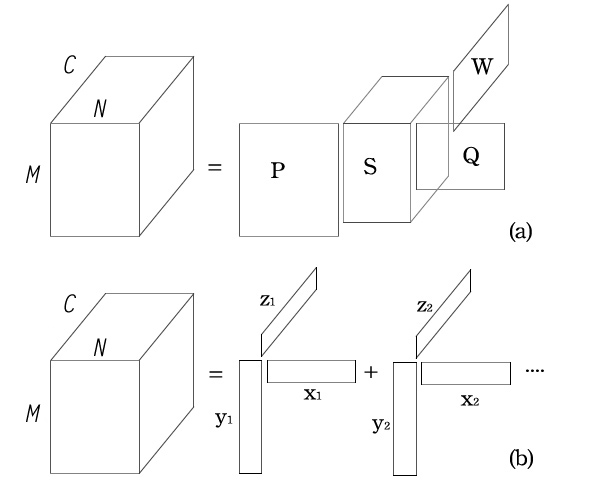
\includegraphics[width=8cm]{tf.jpg} 
%\caption{(a) Tucker Decomposition (TD). (b) Canonical Decomposition, a special case of TD.}
%%In sensor networks, the three dimension can be nominal features such as node id, time step index.} 
%\label{fig:tf:tuckcanon} 
%\end{figure}

\subsubsection{Tensor Factorization for Data Imputation} \label{sec:tfmissing}
%\subsubsection{Objective function}

Existing Tensor Decomposition models assume no missing entries, which is naturally unsuitable for our problem.
Although tensor factorization has been studied for a while and enjoys a certain level of success in building context-aware 
recommender systems~\cite{karatzoglou2010multiverse,rendle2010pairwise}, we have not yet seen any proposal to leverage 
such techniques for sensor data imputation.

Here we introduce Temporally-Regularized Tensor Factorization (TR-TF) model for missing data estimation. 
Similar to TR-MF, TR-TF learns the temporal correlation given the sparsity of data with the capability to take additional information such as spatial correlation and heterogeneous sensor readings into consideration.

We borrow the idea of Canonical Decomposition rather than Tucker Decomposition.
Consider a three-dimensional tensor (e.g., the temperature reading of a sensor given a certain time-stamp and a certain humidity reading), a tensor model can be described as:
\begin{equation*}
%\small
\mbox{Factorization} :=  F_1 \times  F_2 \times F_3 \rightarrow F_1 \times K, F_2 \times K, F_3 \times K
\end{equation*}
Tensor factorization model decomposes the three dimensional tensors T into three matrices. One of them represents the temporal dimension, and the rest can represent sensor nodes, sensor node coordinates, heterogeneous sensor readings, etc. In the experiments, we implemented a three dimensional tensor model and chose the sensor nodes as well as the multivariate sensor readings as the remaining two dimensions.

%In contrast to the conventional tensor decomposition, the factorization model we propose aims at learning the latent factors $\mathbf{P}$,  $\mathbf{Q}$, $\mathbf{W}$ of the three dimensions $F_1, F_2, F_3$.
%To avoid over-fitting and to reduce the complexity of prediction, our model borrows the idea of Canonical Decomposition rather than Tucker decomposition. Note that the time complexity for making a prediction is only $O(K)$, where $K$ is the factor size of $\mathbf{P}$, $\mathbf{Q}$ and $\mathbf{W}$. Thus, the complexity is independent of the size of the tensor, which is a favorable property because we can freely add new dimensions into the model without concerns about prediction efficiency.
%
Similar to the TR-MF model, we also add bias terms to each dimension into the TR-TF model. The prediction function is:
\begin{equation*}
\small
\hat{t}_{mnc}=\mu_m+\mu_n+\mu_c+\sum\limits_{k=1}^{K}{p_{mk} q_{nk} w_{ck}}
\end{equation*}
%To learn the latent factors $\mathbf{P}$, $\mathbf{Q}$ and $\mathbf{W}$, we use the loss function :
%\begin{center}
%$L(\mathbf{\hat{T}},\mathbf{T})=\frac{1}{\|\mathbf{D}\|_1} \sum\limits_{t\in \mathbf{D}}  l(\hat{t},t)$
%\end{center}
%where $\|\mathbf{D}\|$ indicates the size of the observed readings.
%$l$ is a point-wise loss function penalizing the distance between estimate and observation.
%We select $L_2$ norm in our implementation.
%%Ideally $l$ should be as close to the final evaluation metrics (e.g. least square error in our implementation) as possible.
%
%Simply minimizing a loss function is prone to over-fitting. Here we add regularization terms based on the $L_2$ norm to ensure that the model complexity does not grow without bound to avoid over-fitting.
%Similar to our TR-MF model, we also add the time regularization terms into our model.
After adding regularization, the final objective function of tensor factorization becomes :\\
\begin{equation*}
\small
\begin{aligned}
&\sum\limits_{m, n, c} \frac{1}{2}(\hat{t}_{mnc}- t_{mnc})^2\\
+ &\frac{\beta}{2}(\sum_m(\mu_m + \|\mathbf{p}_m\|^2) + \sum_n(\mu_n + \|\mathbf{q}_n\|^2) + \sum_c(\mu_c + \|\mathbf{w}_c\|^2))\\
+ &\frac{\gamma}{2}\sum_m((\mu_m-\mu_{m+1})^2 + (\mathbf{p}_m-\mathbf{p}_{m+1})^2)\\
\end{aligned}
\end{equation*}

%\begin{algorithm}[h]
%  \caption{Temporally-Regularized Tensor Factorization}
%  \label{alg::conjugateGradient}
%  \textbf{Parameter:} $\beta_1,\beta_2, \beta_3, \beta_4, \beta_5, \beta_6, \gamma_1, \gamma_2, \eta, K$
%  \textbf{Input:} training set, validation set
%  \begin{algorithmic}[1]
%    \State Normalize the training set as $\mathcal{D}$
%    \State Initialize $\mu_m, \mu_n, \mu_c, \mathbf{p}_m, \mathbf{q}_n, \mathbf{w}_c $ for all $m, n, c$
%    \Repeat
%      \For {each observed reading $t$ in $\mathcal{D}$}
%     	 \State Update $\mu_m, \mu_n, \mu_c, \mathbf{p}_m, \mathbf{q}_n, \mathbf{w}_c$ 
%      \EndFor
%     \State Update $\mu_m, \mathbf{p}_m$ for all $m$ by temporal regularization
%    \Until stopping criterion is met
%    \State Output the model for testing set prediction 
%  \end{algorithmic}
%\end{algorithm}

\subsubsection{Optimization}
Minimizing the above objective function can be done using many different strategies.
For efficiency and scalability, we suggest Stochastic Gradient Descent~(SGD) as in TR-MF.
Focusing on an observed reading data $T_{mnc} $, the update rules for all $k$s are:
\begin{equation*}
\small
\begin{aligned}
  &p_{mk}^\prime=p_{mk}-\eta(e\times q_{nk}\times w_{ck} + \beta \times p_{mk})
\\&q_{nk}^\prime=q_{nk}-\eta(e\times p_{mk}\times w_{ck} + \beta \times q_{nk})
\\&w_{ck}^\prime=w_{ck}-\eta(e\times p_{mk}\times q_{nk} + \beta \times w_{ck})
\\&{\mu_m}^\prime=\mu_m-\eta(e+\beta\mu_m)
\\&{\mu_n}^\prime=\mu_n-\eta(e+\beta\mu_n)
\\&{\mu_c}^\prime=\mu_c-\eta(e+\beta\mu_c)
\end{aligned}
\end{equation*}
where $e=\hat{t}_{mnc}-t_{mnc}$. After a round of updating, we then update the model according to temporal regularization :
\begin{equation*}
\small
\begin{aligned}
&{\mathbf{p}_m}^\prime={\mathbf{p}_m}-\eta\gamma((\mathbf{p}_m-\mathbf{p}_{m+1})+(\mathbf{p}_m-\mathbf{p}_{m-1}))
\\&{\mu_m}^\prime=\mu_m-\eta\gamma((\mu_m-\mu_{m+1})+(\mu_m-\mu_{m-1}))
\end{aligned}
\end{equation*}
%The Temporally-Regularized Tensor Factorization is summarized in Procedure \ref{alg::conjugateGradient}, which is not hard to implement since it accesses only one row of $\mathbf{P}$, $\mathbf{Q}$, $\mathbf{W}$ at a time.

TR-TF applies similar normalization and stopping criterion techniques as in Section~\ref{sec:mf}.
Its time complexity is also similar to that of TR-MF,
except TR-TF models can be trained even more efficiently because it usually consists of fewer factors and does not require many iterations to converge. 
%Empirically, one can achieve reasonable performance by imposing the following constraints on the parameter learning:  
%\begin{equation*}
%$\beta_1=\beta_2=\beta_3=\beta_4=\beta_5=\beta_6$ \mbox{ and } $\gamma_1=\gamma_2$.
%\end{equation*}
